% METODOLOGIA

\chapter{SISTEMA DE ATUALIZAÇÃO DE FIRMWARE OVER-THE-AIR}
\label{chap:metodologia}
Nesse capitulo é retratado como será o funcionamento do sistema que será desenvolvido, mostrada uma visão geral do projeto, listadas as funcionalidades de cada uma das partes do \textit{software}, explicando sua atividade, sua implementação, e as ferramentas utilizadas para o seu teste e os materiais utilizados. 

\section{VISÃO GERAL}
O \textit{software} que será desenvolvido nesse trabalho é dividido em duas partes, uma contendo o \bootloader, com o auxílio da biblioteca FatFs, realizará a comunicação com o cartão SD, que conterá o novo \firmware\ previamente recebido. Assim poderá substituir o \software\ anterior da aplicação por um novo. Essa parte do \software\ ficará armazenada em uma região da memória que dificilmente será reescrita, podendo ser reescrita somente com o auxílio de ferramentas de desenvolvimento como um JTAG e/ou \textit{debugger}, então é uma peça do programa que improvavelmente será substituída. Será uma parte que é portável para todos os microcontroladores da familia STM32, pois faz uso direto de funções de escrita na memória flash obtidas por meio do STM32Cube HAL, ficando a cargo do projetista fazer um pequeno porte que posteriormente será explicado neste trabalho.

A outra parte desse trabalho será uma API, contendo as demais funções necessárias para a comunicação com o servidor, que enviará para o sistema o novo \firmware, por meio do uso da biblioteca LwIP, garantirá a segurança dessa conexão com a utilização de uma camada extra de proteção, com biblioteca Mbed TLS. Essa API irá conectar-se a um servidor, em que verificará a disponibilidade de uma nova versão de \software. 

Após ser confirmada a existência de uma nova versão de \firmware, a API irá se comunicar novamente com o servidor com o intuito de fazer o \download\ dessa nova versão, e a armazenar no cartão SD do sistema. Com o download concluído com sucesso a API se conectará novamente com o servidor para obter o arquivo contendo o hash deste firmware, ela então executará uma função que cria um hash para o \firmware\ baixado e o compara com arquivo de hash obtido do servido, para assim garantir que o firmware está integralmente no cartão sd. Então o \bootloader\ entre em ação após uma reinicialização do sistema. De forma geral o funcionamento do sistema pode ser observado na \autoref{fig:visaogeral}

\begin{figure}[H]
    \scriptsize
     \centering
     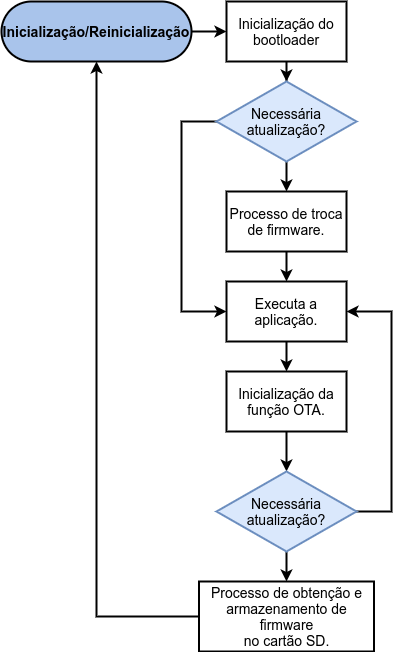
\includegraphics[scale=0.8]{dados/figuras/FuncionamentoGeral.png}
     \caption{Visão geral do funcionamento do sistema de atualização. \newline Fonte: autoria própria.}
     \label{fig:visaogeral}
\end{figure}

A API será uma peça de \software\ que poderá ser substituída e atualizada em conjunto com as demais aplicações do sistema, como, as bibliotecas LwIP, Mbed TLS, o sistema operacional, entre outras peças de \software\ utilizadas pela aplicação. 
O sistema de atualização OTA utiliza-se de bibliotecas já conhecidas e vastamente utilizadas por desenvolvedores de sistemas embarcados. Assim projetos que necessitem fazer comunicação segura via rede, leitura e escrita de cartões SD, possam utilizar esse sistema de modo a poupar espaço na memória, visando a reutilização dessas bibliotecas. Portanto, o sistema pode ser amplamente utilizado por sistema de IoT. 
%Será utilizada o \textit{kit} de desenvolvimento STM32F746G \textit{Discovery}, onde será inicialmente desenvolvida a API, suas tarefas e o \textit{bootloader} que serão os principais componentes desse sistema.

Em caso de uma falha durante o processo de atualização OTA, o sistema tem a habilidade de se recuperar de forma autónoma. Como não haverá sobreescrita na área em que o \textit{firmware} está posicionado no cartão SD, uma simples reinicialização do sistema pode fazer com que o bootloader seja ativado novamente e refaça o processo de cópia da memória.

%O sistema de atualização irá funcionar da seguinte forma, após a inicialização do sistema o \bootloader\ é executado e verifica a existência de um novo \firmware, no caso negativo ele inicia normalmente o \software\ principal da aplicação. No caso positivo, o \bootloader\ inicia o processo de substituição de \textit{firmware}, após a troca, o novo \software\ é iniciado. Durante a execução da aplicação principal do sistema e em um tempo determinado pelo projetista, a API entra em contato com o servidor para verificar a disponibilidade de um \software\ novo, em caso positivo ela agenda um período para a atualização do \firmware, no caso negativo ele continua a execução da aplicação. 

%Caso haja uma atualização quando o horário do agendamento chegar, a API irá conectar-se ao servidor e iniciar o processo de \download\ do \firmware\ novo e armazená-lo em uma área já predefinida do cartão SD para que o \bootloader\ possa o encontrar. Após o \download\ o sistema será reiniciado e o \bootloader\ entrará será executado novamente. 
%De forma resumida o funcionamento do sistema pode ser visto na \autoref{Funcionamento}, 


%Com a  As tarefas serão produzidas a partir de b
%sistema possa conter intersecções com trechos de codigos utilizados em varios projetos que necessitam

%Adicionar diagrama de blocos!!!!

% A seguir será explicado parcialmente como funcionarão as funções das tarefas, do \textit{bootloader}, e do servidor HTTP.
%Cada capítulo deve conter uma pequena introdução (tipicamente, um ou dois parágrafos) que deve deixar claro o objetivo e o que será discutido no capítulo, bem como a organização do capítulo.

\section{\textit{BOOTLOADER}}
\label{sec:Bootloader}

A partir de um arquivo de \textit{linker}, a memória da plataforma será customizada com o intuito de abrigar os arquivos necessários para o \bootloader\ e protegê-lo de eventuais sobrescritas que podem vir a ocorrer. Esse arquivo de \textit{linker}, assim como o próprio \textit{bootloader}, será escrito somente para os microcontroladores da familia STM32, visto que cada plataforma tem suas próprias características como, tamanho de memória e endereços diferentes para cada fabricante e/ou arquitetura.

No arquivo de \linker\ será especificada uma área especial na memória flash do sistema em que será abrigado o \bootloader. Também será responsável por fazer com que o \bootloader\ seja chamado após a inicialização do sistema. Assim será garantido que o \bootloader\ sempre entre seja executado após a reinicialização do sistema embarcado.

%irá verificar o \textit{hash} da nova versão, verificando a integridade e origem do \textit{software},

O \textit{bootloader} será responsável em fazer a troca de cada versão de \textit{firmware} instalado no sistema embarcado. Sempre que o sistema for iniciado, o \textit{bootloader} será inicializado e fará a procura de arquivos. Essa busca será possível pelo fato da biblioteca FatFs, que está implementada junto ao \bootloader, criar um sistema de arquivos no cartão SD do sistema alvo, assim o \bootloader\ pode acessar a memória do cartão sem a necessidade da aplicação final ser inicializada.

Se após o \textit{reset} a procura do arquivo contendo a versão do \firmware\ novo retornar com um resultado positivo, ele converte o valor contido neste arquivo de uma string para um tipo inteiro e o compara com os quatro últimos bytes da memória flash, posição onde se encontra a versão atual do \firmware , caso a versão do novo firmware seja maior que a do firmware atual o \bootloader\ inicia o processo de atualização.

Nesse processo o \bootloader\ substitui completamente o \textit{firmware} e demais bibliotecas e API's em áreas não protegidas na memória, pelo binário do \textit{firmware} presente no cartão SD. Esse processo é implementado com o uso das funções de escrita na memória flash do HAL fornecido pela STM32, onde inicialmente é feito o processo de apagamento massivo dos setores da aplicação da memória flash, dessa forma esses setores são preenchidos com o valor 0xFF em cada byte.

Após o processo de apagamento é iniciado o processo de escrita, em que o arquivo contendo o firmware é lido a cada 512 bytes para um buffer, e a partir deste buffer são escritos 4 bytes por vez na memória flash, assim esse processo se repete até que o arquivo contendo o novo firmware seja completamente escrito na memória.
Finalizada a escrita do novo firmware, acontece a escrita da versão nos quatro últimos bytes da memória somente após essa escrita o processo de atualização pode ser considerado concluído com sucesso, e então ele pode apagar do cartão SD os arquivos do firmware e versão.

Caso o bootloader seja iniciado e em algum momento detectar que o valor dos quatro ultimos bytes são iguais a 0xFFFFFFFF, ele identifica que a ultima operação de atualização não foi concluída com exito. Neste estado o bootloader fica sempre tentando encontrar uma nova versão do \firmware\ no cartão SD e caso não encontre ele fica reiniciando o microcontrolador, e caso ele encontre ele tenta atualizar novamente como o firmware encontrado, independente da versão dele, garantindo assim que o sistema seja resistente a eventuais erros e eventos não previstos, como quedas de energia durante o processo. O funcionamento do \textit{bootloader} pode ser observado na \autoref{fig:DiagBootloader}.

\begin{figure}[H]
    \scriptsize
     \centering
     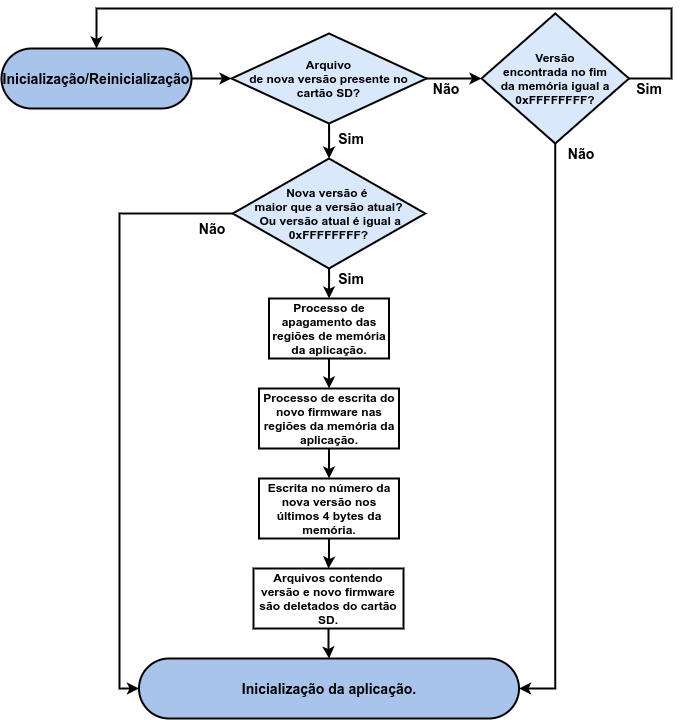
\includegraphics[scale=0.6]{dados/figuras/FuncionamentoBootloader.png}
     \caption{Diagrama de funcionamento do \bootloader. \newline Fonte: autoria própria.}
     \label{fig:DiagBootloader}
\end{figure}
%Inserir seu texto aqui...

%\section{SERVIDOR HTTP}
%\label{sec:ServidorHTTP}

%A partir de um computador conectado à mesma rede que o sistema embarcado, haverá um servidor HTTP que ficará responsável por esperar requisições do dispositivo, para consultar a disponibilidade de uma versão atualizada do \textit{software}, e após a confirmação dessa nova versão, esse servidor irá enviar o \textit{firmware} para a plataforma embarcada.
%Inserir seu texto aqui...

\section{API DE ATUALIZAÇÃO OTA}
\label{sec:API}

A API de atualização OTA que foi desenvolvida nesse trabalho tem o propósito de ser o mais portável possível, para assim, ser reutilizada por diversos projetos que necessitem da troca de seu \software\ e com isso pode ser chamada quando o desenvolvedor necessitar, como após uma interrupção externa ou comando do servidor. Com esse objetivo, serão utilizadas as bibliotecas já bem difundidas, a LwIP para a criação da pilha TCP/IP, a Mbed TLS para criar uma camada se segurança nessa pilha, e a FATFS para a criação de um sistema de arquivos FAT. Assim desenvolvedores podem se aproveitar do fato de que essas bibliotecas já estão em seus sistemas como padrão para utilizá-las em suas próprias funcionalidades. 
A seguir será retratado como serão cada uma das funcionalidades necessárias na API.

\subsection{COMUNICAÇÃO COM O SERVIDOR}

Com o uso da biblioteca LwIP e Mbed TLS foi criada uma pilha de comunicação no sistema alvo, que é responsável pela conexão segura com o servidor que fornecerá o novo firmware. Na implementação da pilha de comunicação, foi utilizada a API BSD Sockets, pois, o intuito é deixar o sistema de atualização portável, e essa API fornece suporte a sistemas operacionais de tempo real entre outra vantagens.

Como a biblioteca Mbed TLS já foi desenvolvida para ser integrada facilmente a várias aplicações embarcadas, ela foi utilizada para criar protocolos de segurança nessa comunicação com o servidor. Foram utilizados padrões SSL/TLS para ser criado um canal criptografado entre o servidor e o sistema alvo, para garantir que todos os dados transmitidos sejam sigilosos e seguros.

A comunicação com o servidor será feita por meio de um servidor HTTP que utilizará o protocolo TCP para garantir que todos os dados obtidos pelo servidor sejam integros, evitando que o novo \textit{firmware} e demais dados obtidos sejam corrompidos. 

%essa tarefa estará responsável por criar uma comunicação segura entre o \textit{hardware} e o servidor HTTP, a partir dessa comunicação será feito a verificação do sinal de disponibilidade de novo \textit{software} e \textit{download} do mesmo quando o sistema estiver ocioso. 

\subsection{DOWNLOAD E ARMAZENAMENTO DO FIRMWARE}

A partir da utilização da biblioteca FatFs, será criado um sistema de arquivo FAT, que gerenciará a memória presente no cartão SD dentro da aplicação, e ele pode ser utilizado tanto pela aplicação final do sistema embarcado, quanto pela API. Esse sistema de arquivo será utilizado para que se possa identificar a posição na memória em que o \textit{firmware} novo será colocado após o seu \download, evitando que outros arquivos, pertencentes a aplicação final, sejam colocados com o mesmo nome, e fazendo com que o \bootloader\ interprete de forma errada os arquivos gerando erros.

Quando o desenvolvedor iniciar a função OTA, a API iniciará novamente a comunicação com o servidor que contém o \textit{firmware} novo, dessa vez com o propósito de fazer \download\ do arquivo contendo o numero da nova versão do \textit{software}. Após o \download\ a API ainda irá verificar se o valor obtido por meio deste arquivo é maior que o presente nos últimos 4 bytes da memória, para assim verificar se existe a necessidade de se continuar com o processo de atualização. 

Caso o valor da nova versão seja maior que a versão atual do firmware a API inicia o \download\ do novo firmware, após esse processo a ferramenta inicia a comunicação novamente para obter agora o arquivo contendo o hash do firmware posteriormente baixado, e com isso é feito um teste de integridade neste firmware onde inicialmente se gera um hash a partir do algoritmo SHA-256 fornecido pela biblioteca MBED TLS, e esse hash é comparado com aquele baixado do servido. Se esse teste retornar com sucesso o processo de atualização é continuado, e o arquivo de hash baixado do servidor é apagado do cartão SD e é iniciado o processo de reinicialização do microcontrolador com o intuito de se iniciar o bootloader para completar o processo de atualização.
A \autoref{fig:DiagAPI} ilustra o funcionamento da API.

\begin{figure}[H]
    \scriptsize
     \centering
     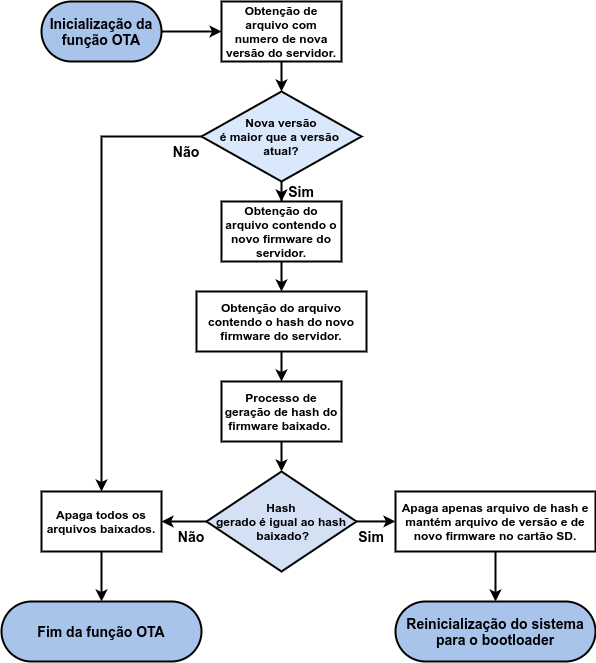
\includegraphics[scale=0.75]{dados/figuras/FuncionamentoAPI.png}
     \caption{Diagrama de funcionamento da API.\newline Fonte: autoria própria.}
     \label{fig:DiagAPI}
\end{figure}
%maquina de estado para leitura do arquivo.
\section{MATERIAIS UTILIZADOS}

A API e o bootloader foi escrito na linguagem C, enquanto o \linker\ será escrito em comandos de \linker. A escrita desses códigos será feita com o uso do ambiente de desenvolvimento integrado Eclipse \cite{Eclipse}. O sistema de atualização OTA desenvolvido nesse trabalho é inicialmente desenvolvido para a plataforma STM32F746G-Discovery.

\subsection{PLATAFORMA STM32F746G-DISCOVERY}

O STM32F7 Discovery é um kit de desenvolvimento que permite ao usuário desenvolver e compartilhar aplicações com toda a série de microcontroladores STM32F7 baseados no processador ARM\textregistered  Cortex\textregistered-M7 core.
O kit discovery permite uma ampla diversidade de aplicações que podem se beneficiar de suporte a múltiplos sensores, áudio, tela gráfica, segurança, vídeos e conexões de alta velocidade \cite{STM32F7}.
A \autoref{STM32F7} ilustra o kit STM32F746NGH6-Discovery.

\begin{figure}[H]
    \scriptsize
     \centering
     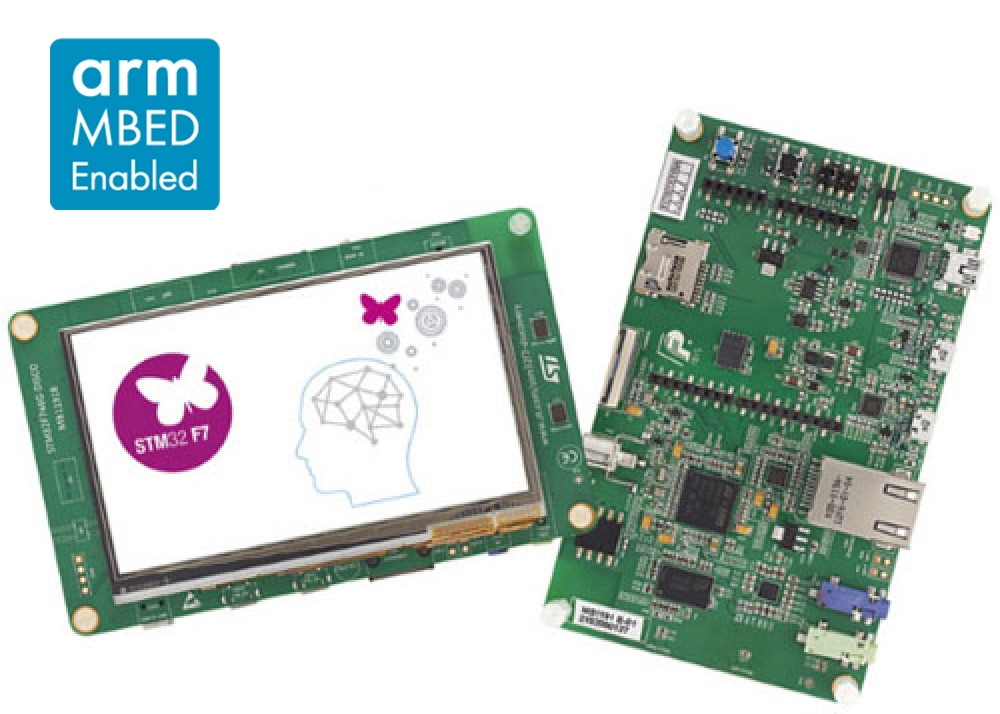
\includegraphics[scale=0.4]{dados/figuras/STM32F7.jpg}
     \caption{Kit de desenvolvimento STM32F746G-Discovery. \newline Fonte:\cite{STM32F7}.}
     \label{STM32F7}
\end{figure}

Algumas de suas principais características são \cite{STM32F7}:
\begin{itemize}
    \item Microcontrolador STM32F746NGH6 com 1 Mbytes de memória flash e 340 Kbytes de RAM, em um pacote BGA216.
    \item 128-Mbit de memória Quad-SPI Flash.
    \item 128-Mbit SDRAM (Com 64 Mbits Acessível).
    \item Conector para cartão microSD.
    \item Conector Ethernet em conformidade com a IEEE-802.3-2002
    \item Tela LCD de 4,3 polegadas, com resolução de 480x272 com \textit{touch-screen} capacitivo.
    
\end{itemize}

\subsection {FIRMWARES DE TESTE PROPOSTOS}
Para os testes apresentados neste trabalho foram desenvolvidos três firmwares muito parecidos, ambos possuem todas as bibliotecas necessárias para que sistema de atualização OTA proposto funcionem corretamente, além de possuírem o sistema operacional de tempo real FreeRTOS. Esses firmwares foram desenvolvido para somente darem suporte ao sistema e não exercerem nenhuma outra função, então temos uma estimativa do tamanho que somente o sistema de atualização, suas bibliotecas e o FreeRTOS ocupam em memória.

Esses firmwares contém em sua função main, além de inicializações necessárias de drivers, bibliotecas e do sistema operacional, uma pequena função que apresenta uma mensagem de apresentação mostrando a versão do firmware atual e uma mensagem de teste somente para fazer uma diferenciação entre as versões e como mostrada na \autoref{mensagemteste}. 

\begin{figure}[H]
    \scriptsize
     \centering
     
\includegraphics[scale=1.2]{dados/figuras/ToDo.jpg}
     \caption{As três mensagens exibidas para diferenciação dos \firmware. \newline Fonte: Autoria própria.}
     \label{mensagemteste}
\end{figure}

A função padrão destes firmware é um laço infinito que a cada XXXX segundos inicializa a função OTA que inicializa o processo de atualização, assim temos uma garantia que o firmware ira sempre ficar executando a funçao OTA.